%----------------------------------------------------------------------------
%----------------------------------------------------------------------------
On the conditioning table we delay and spatially filter the three dye laser beams. The delay line is a rail with a sliding ``car'' which the user moves by hand. With the beam line folded four times, we can achieve delays of $\pm$ 8 ns using a 4 foot rail. It will only be necessary to delay two of the beams (dye lasers \#22 and \#23) to generate arbitrary pulse sequences with internal delays less than 8 ns. After the beams are synchronized, we spatially filter each beam using a pinhole. The filter consists of a focusing lens, high damage threshold pinhole, and a collimating lens to capture the usable portion of the pinhole output. See figure \ref{conditioning_table}.
%----------------------------------------------------------------------------
% conditioning_table.tex
% by Troy Hix, May 2005
%----------------------------------------------------------------------------
\begin{sidewaysfigure}
\center
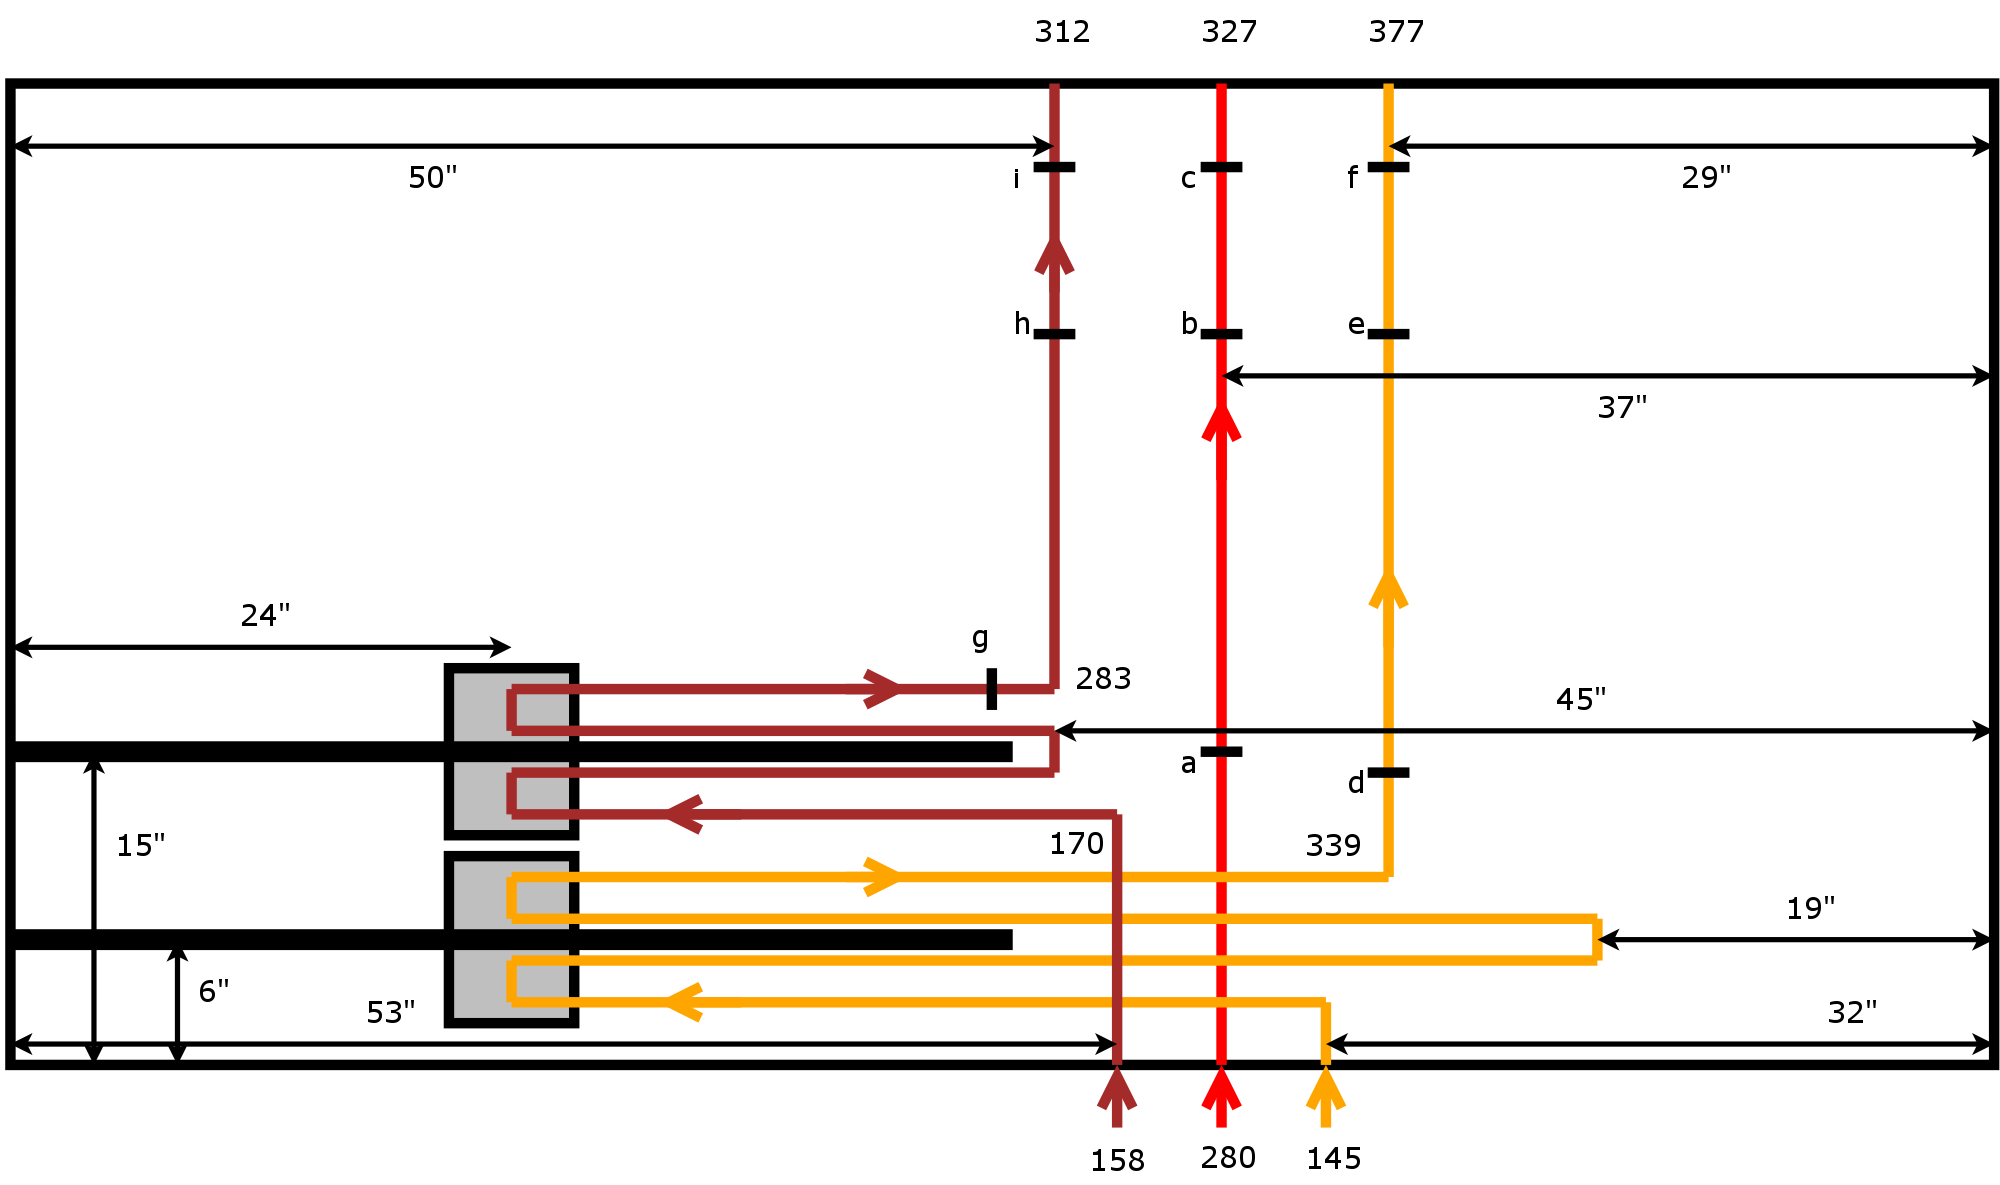
\includegraphics[width=7.75in]
{conditioning_table/conditioning_table.png}\\
\caption[Beam conditioning table]{Beam conditioning table. (a) is a +0.5 m lens at milepost 295, (b) is a pinhole at milepost 315.3, (c) is a +0.2 m lens at milepost 323.2, (d) is a +0.5 m lens at milepost 344, (e) is a pinhole at milepost 364.7, (f) is a +0.2 m lens at milepost 372.5, (g) is a +0.5 m lens at milepost 280, (h) is a pinhole at milepost 300.3, and (i) is a +0.2 m lens at milepost 308.2. The delay lines are shown as horizontal black bars; the delay ``cars'' (in the zero delay position) are shown as gray rectangles.}
\label{conditioning_table}
\end{sidewaysfigure} 
%----------------------------------------------------------------------------
%----------------------------------------------------------------------------
%----------------------------------------------------------------------------



%----------------------------------------------------------------------------
%----------------------------------------------------------------------------
%----------------------------------------------------------------------------
%----------------------------------------------------------------------------
%----------------------------------------------------------------------------
